\chapter{Magnetismo de sólidos} \label{Ch:10}

En este Capítulo se estudian algunas de las contribuciones más importantes al magnetismo de los sólidos. Como se verá, alguna de ellas (como la ferromagnética) constituye un fenómeno cooperativo que lleva asociado una transición de fase. Es también destacable que el magnetismo de sólidos es en buena medida un efecto cuántico dado que muchas de sus causas (el momento mangnético de espín, la interacción de intercambio, etc.) no tienen análogo clásico.

\section{Relaciones básicas}

La \textbf{magnetización} (o imanación) $\Mn$ se define como el momento magnético por unidad de volumen 

\begin{equation}
	\Mn = \frac{1}{V} \sum_V \mun	
\end{equation}
donde los $\mun$ son los momentos magnéticos atómicos o iónicos en el ``volumen de control'' $V$. Recordemos que para partículas sin espín $\mun =  \sum_i \frac{1}{2} \rn_i \times q_i \vn_i$ y que para \textit{lazos} de corriente $\mun  = I \An$ siendo $I$ la intensidad y  $\An$ el área encerrada. El magnetismo de los sólidos se clasifica de acuerdo a la interrelación de su magnetización con el campo magnético aplicado $\Hn$. Así, se introduce la \textit{susceptibilidad magnética} $\chi$ por 

\begin{equation}
	\Mn = \chi \Hn
\end{equation}
En general $\chi$ será un tensor, pero no consideraremos esta complicación aquí. Si un medio tiene $\chi$ negativa se el sólido se dice \textit{diamagnético} y si por contra $\chi$ es positiva el sólido se dice \textit{paramagnético}. Además, existe un grupo de materiales que pueden poseer magnetización aun en ausencia de campo aplicado y que son \textit{ferromangéticos} (observar que $\chi \rightarrow \infty$).

\section{Diamagnetismo atómico}

La naturaleza del diamagnetismo atómico se puede comprender a partir de un modelo clásico en que cada órbita electrónica es considerada una espira de corriente. De acuerdo con la ley de Lenz, al variar el flujo magnético sobre el circuito surge una fuerza electromotriz de inducción que hace variar la corriente y por tanto genera un momento magnético adicional. Así, si $A$ es el área de la órbita, $\omega$ la velocidad angular e $I$ la intensidad de corriente, el momento magnético será $\mu=IA=-(e\omega / 2\pi)A$, y bajo la aplicación de un campo $B$ perpendicular a la órbita, aquél se incrementa en

\begin{equation}
	\Delta \mu = - \frac{eA}{2\pi} \Delta \Omega \label{Ec:10-02-01}
\end{equation}
La variación de velocidad angular $\Delta \omega$ se determina del balance de fuerzas sobre la órbita, que consideramos circular de radio $r$ (ver figura \ref{Fig:10-01}): antes de la aplicación del campo de fuerza nuclear se equipara a la fuerza centrífuga, $F_\text{núcleo} = m\omega^2 r$; tras la aplicación del campo aparece adicionalmente la fuerza de Lorentz $F_L = ev B$ dirigida hacia el núcleo, que se compensa con un aumento de la velocidad angular 

\begin{equation}
	m(\omega + \Delta \omega)^2 r = F_\text{núcleo} + e v B
\end{equation}
Como para los campos magnéticos aplicables en un laboratorio $evB\ll m \omega^2 r$, se tiene que $\Delta \omega \ll \omega$. Así pues, despreciando términos en $\Delta \omega^2$ se deduce 

\begin{equation}
	\Delta \omega = \frac{evB}{2mr\omega} = \frac{eB}{2m}
\end{equation}
que se denomina \textit{frecuencia de Larmor}. Combinando con (\ref{Ec:10-02-01}) y generalizando a un átomo de $Z$ electrones:

\begin{equation}
	\Delta \mu = - Z \frac{e^2A}{4\pi m} B = - Z \frac{e^2 \langle \rho^2 \rangle}{4m}B
\end{equation}
siendo $\langle \rho^2 \rangle = \langle x^2 + y^2 \rangle = \langle x^2 \rangle + \langle y^2 \rangle$ el valor cuadrático medio de la distancia de los electrones al eje que pasa por el núcleo paralelamente al campo (eje $z$). Si admitimos simetría esférica, $\langle x^2 \rangle=\langle y^2 \rangle=\langle z^2 \rangle$ y con ello el radio cuadrático medio atómico resulta $\langle r^2 \rangle\= \frac{3}{2} \langle \rho^2 \rangle$. Llamando $n$ al número de átomos por unidad de volumen la magnetización resultante es

\begin{equation}
	M = n \Delta \mu = - \frac{nZe^2 \langle r^2 \rangle}{6m}B
\end{equation}
y la susceptibilidad magnética 

\begin{equation}
	\chi = \frac{M}{H} \approx \frac{mu_0 M}{B} = - \frac{\mu_0 n Z e^2 \langle r^2 \rangle}{6m}
\end{equation}
que es el resultado clásico de \textit{Langevin}. Aunque en general $B=\mu_0 (H+M)$, aquí se ha aproximado $B\approx \mu_0 H$ dado que $|M|\ll H$ (o bien que $|\chi |\ll 1$). En efecto, para $n=5\times10^{28} \unit{m}^{-3}$ y $r=10^{-10}$ m, $\chi = -10^{-6}Z$. El diamagnetismo atómico es propio de \textit{todos los cuerpos sin excepción}, aunque a menudo está enmascarado por el paramagnetismo o el ferromagnetismo.

\begin{figure}[h!] \centering
	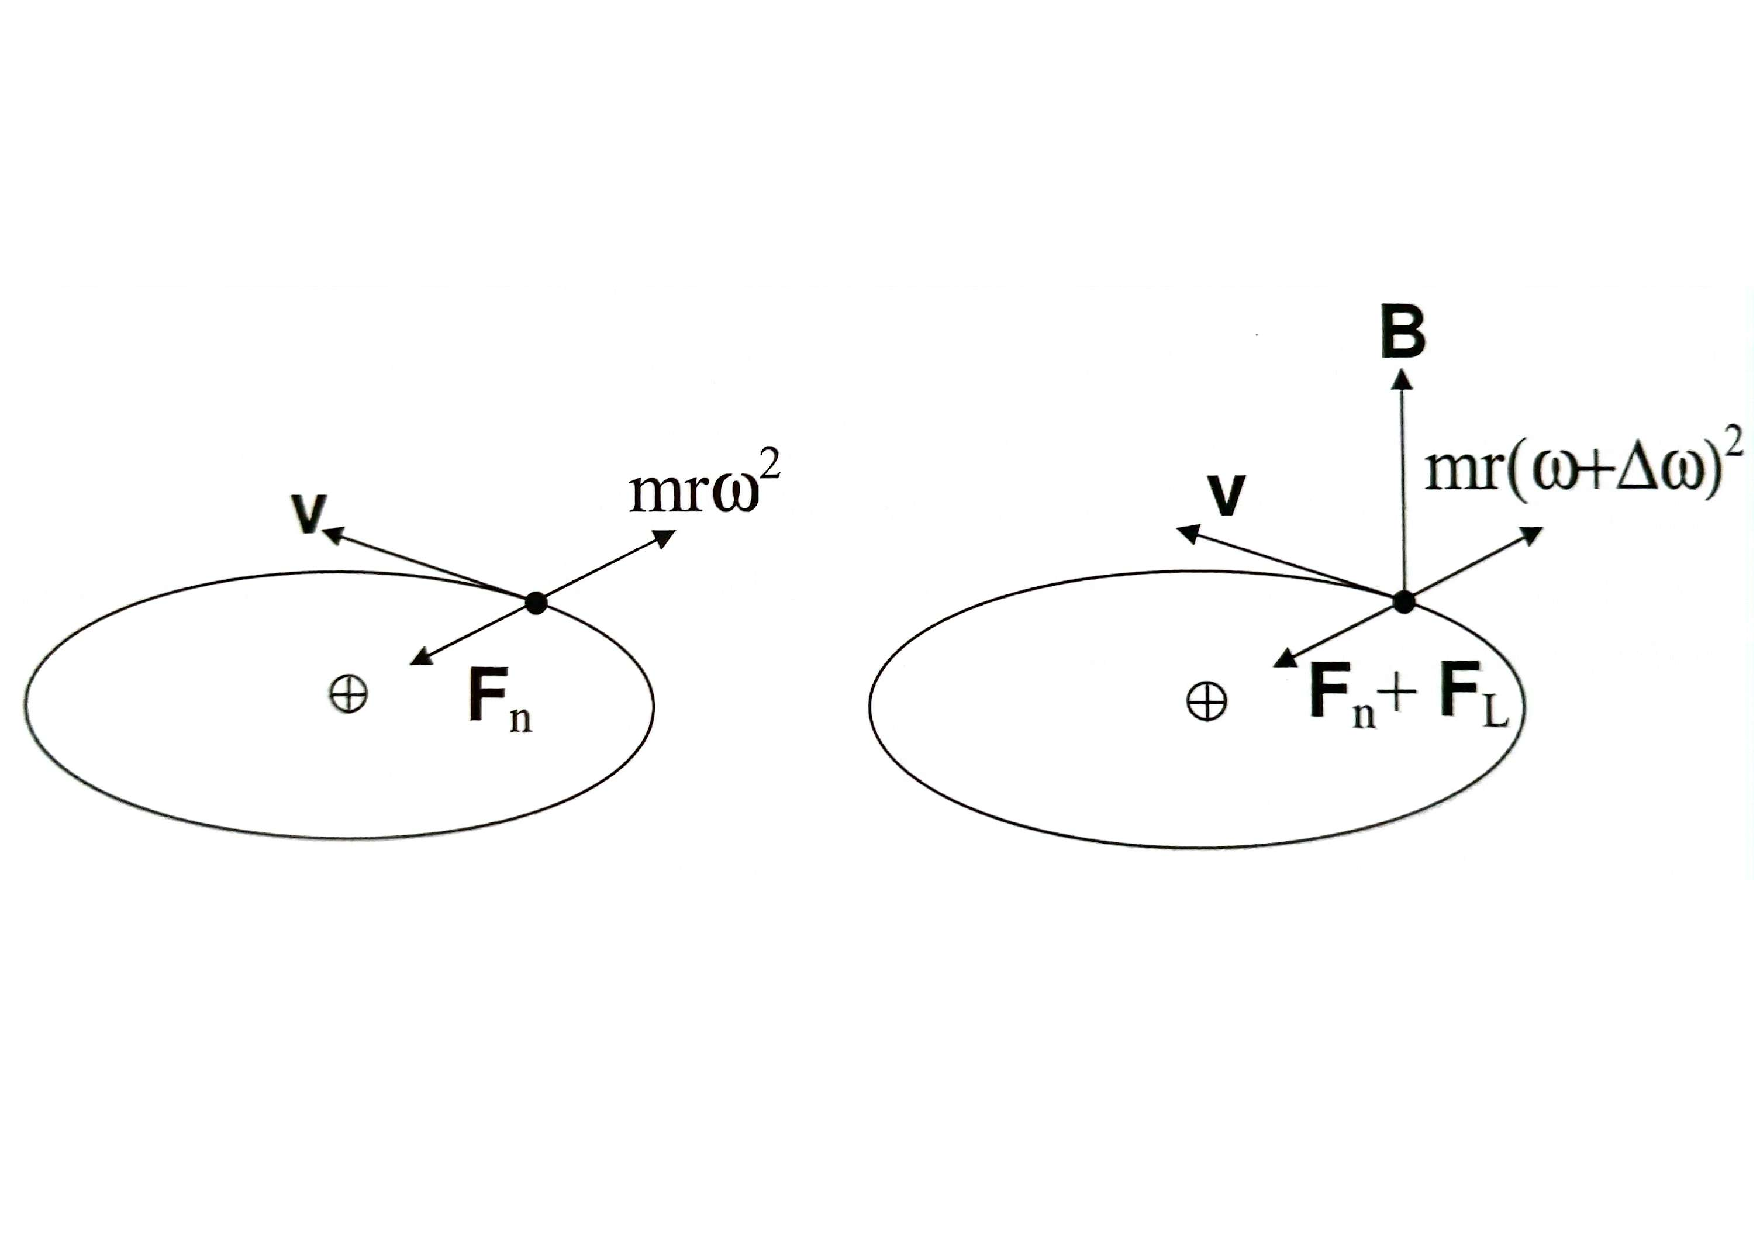
\includegraphics[scale=0.35]{Cuerpo/Ch_10/Fotos libro 1.pdf}
	\caption{Balance  de fuerzassobre un electrón orbitando en torno a un núcleo en ausencia (izquierda) o en presencia (derecha) de un campo mangético externo. El referencial usado es uno centrado en el núcleo y que gira con el electrón de modo qeu hay que considerar las fuerzas inerciales (aquí sólo hay fuerza centrífuga).}
	\label{Fig:10-01}
\end{figure}

\section{Paramagnetismo atómico}

Además de la contribución diamagnética ya vista en la sección anterior, algunos átomos presentan un momento magnético \textit{permanente} debido al espín y al momento angular orbital de los electrones (los momentos magnéticos nucleares son $\sim 10^3$ veces más pequeños y no se tendrán en cuenta). En ausencia de un campo externo los momentos magnéticos atómicos están orientados al azar y la magnetización resultante es nula. Sin embargo, como se verá, bajo la aplicación de un campo magnético los momentos atómicos se orientan en su mismo sentido dando lugar a una mangnetización (\textit{paramagnética}), que puede ser mucho mayor que la diamagnética.

\subsection{Origen del momento mangnético atómico}

El momento mangético orbital electrónico $\mun_L$ se relaciona con el momento angular orbital $\hbar \Ln$ por 

\begin{equation}
	\mun_L \equiv - \frac{e}{2m} \rn \times \pn = - \mun_B \Ln
\end{equation}
donde $\mu_B=e\hbar / 2m=9.3\times 10^{-24}$ J/T es el llamado \textit{magnetón de Bohr}. Los momentos magnéticos magnéticos de espín $\mun_S$ están relacionados con el momento angualr de espín $\hbar \Sn$ por:

\begin{equation}
	\mun_S = - g_0 \mu_B \Sn  \label{Ec:10-03-02}
\end{equation}
siendo $g_0 \approx 2$. Como para un solo electrón $S=1/2$, $\mu_B$ es interpetrable como el momento mangético de espín de un electrón libre. En el caso atómico (varios electrones con contribución orbital y de espín) el momento magnético total $\mun$  también resulta ser proporcional al momento angular electrónico total $\hbar\Jn=\hbar \Ln + \hbar \Sn$ según 

\begin{equation}
	\mun = - g \mu_B \Jn 
\end{equation}
donde 

\begin{equation}
	g = 1 + \frac{J(J+1)+S(S+1)-L(L-1)}{2J(J+1)}
\end{equation}
es el llamado \textit{factor de Landé}. El momento magnético asociado a átomos e iones con capas electrónicas cerradas es nulo. Si existen capas electrónicas interiores parcialmente desocupadas (elementos de transición, tierras raras y actínidos), o capas de valencia con número impar de electrones el momento magnético es distinto de cero. El cálculo de $L,S$ y $J$ del estado atómico fundamental a partir de los momentos angulares electrónicos individuales se hace por las reglas de Hund:

\begin{enumerate}
	\item $S$ toma el valor más alto posible compatible con el principio de exclusión (momentos magnéticos de espín paralelos).
	\item $L$  toma el máximo valor compatible con este valor de $S$ (momentos magnéticos paralelos).
	\item $J=|L-S|$ para una capa llena a menos de la mitad, y $J=L+S$ si a más de la mitad.
\end{enumerate}

\subsection[Dependencia de la magnetización respecto $\vec{\Bn}$ y $T$]{Dependencia de la magneteización paramagnética con la temperatura y el campo magnético}

Los niveles de energía de un momento magnético $\mun$ en un campo de inducción $\Bn$ en la dirección de $z$ se expresan por 

\begin{equation}
	U = - \mun \cdot \Bn = g \mu_B \Jn \cdot \Bn = g \mu_B J_z B \tquad \mu_z = g \mu_B J_z
\end{equation}
donde $J_z = - J_1,...,J$ es el \textit{número cuántico azimutal o magnético}. Queremos calcular el valor medio de $J_z$ (las componentes no paralelas al campo promedian a cero). Estadísticamente la ocupación relativa de niveles a temperatura $T$ la da el factor de Boltzmann $\exp (-U/k_B T)=\exp \parentesis{-g\mu_B J_z B / k_B T}$, de modo que la magnetización neta $M$ de un conjunto de momentos magnéticos \textit{independientes} con una concentración $n$ vendrá dada por 

\begin{equation}
	M = n \frac{\sum_{J_z=-J}^{+J} - g\mu_B J_z \exp \parentesis{- g\mu_B J_z B / k_BT}}{\sum_{J_z=-J}^{+J} \exp \parentesis{-g\mu_B J_z B / k_B T}} \label{Ec:10-03-07}
\end{equation}
tras algunas manipulaciones la suma anterior se iguala a 

\begin{equation}
	M = n g \mu_B J B_J (x)
\end{equation}
donde 

\begin{equation}
	B_J (x) = \frac{2J+1}{2J} \coth \parentesis{\frac{2J+1}{2J}x} - \frac{1}{2J} \coth \parentesis{\frac{x}{2J}} \quad x \equiv \frac{g\mu_B J B }{k_B T}
\end{equation}
es la \textbf{función de Brilluoin}. $B_J$ crece linealmente con $x$ para $x\ll 1$ y satura a q para valores altos de $x$. Por tanto $M$ tiene a la magneteización de saturación a campos $B$ altos correspondiendo al máximo alineamiento de los dipolos con el campo $J_z = -J$. La figura \ref{Fig:10-02} ilustra la variación de $B_J(x)$ y de la magnetización paramagnética para distintos $J$.

\begin{figure}[h!] \centering
	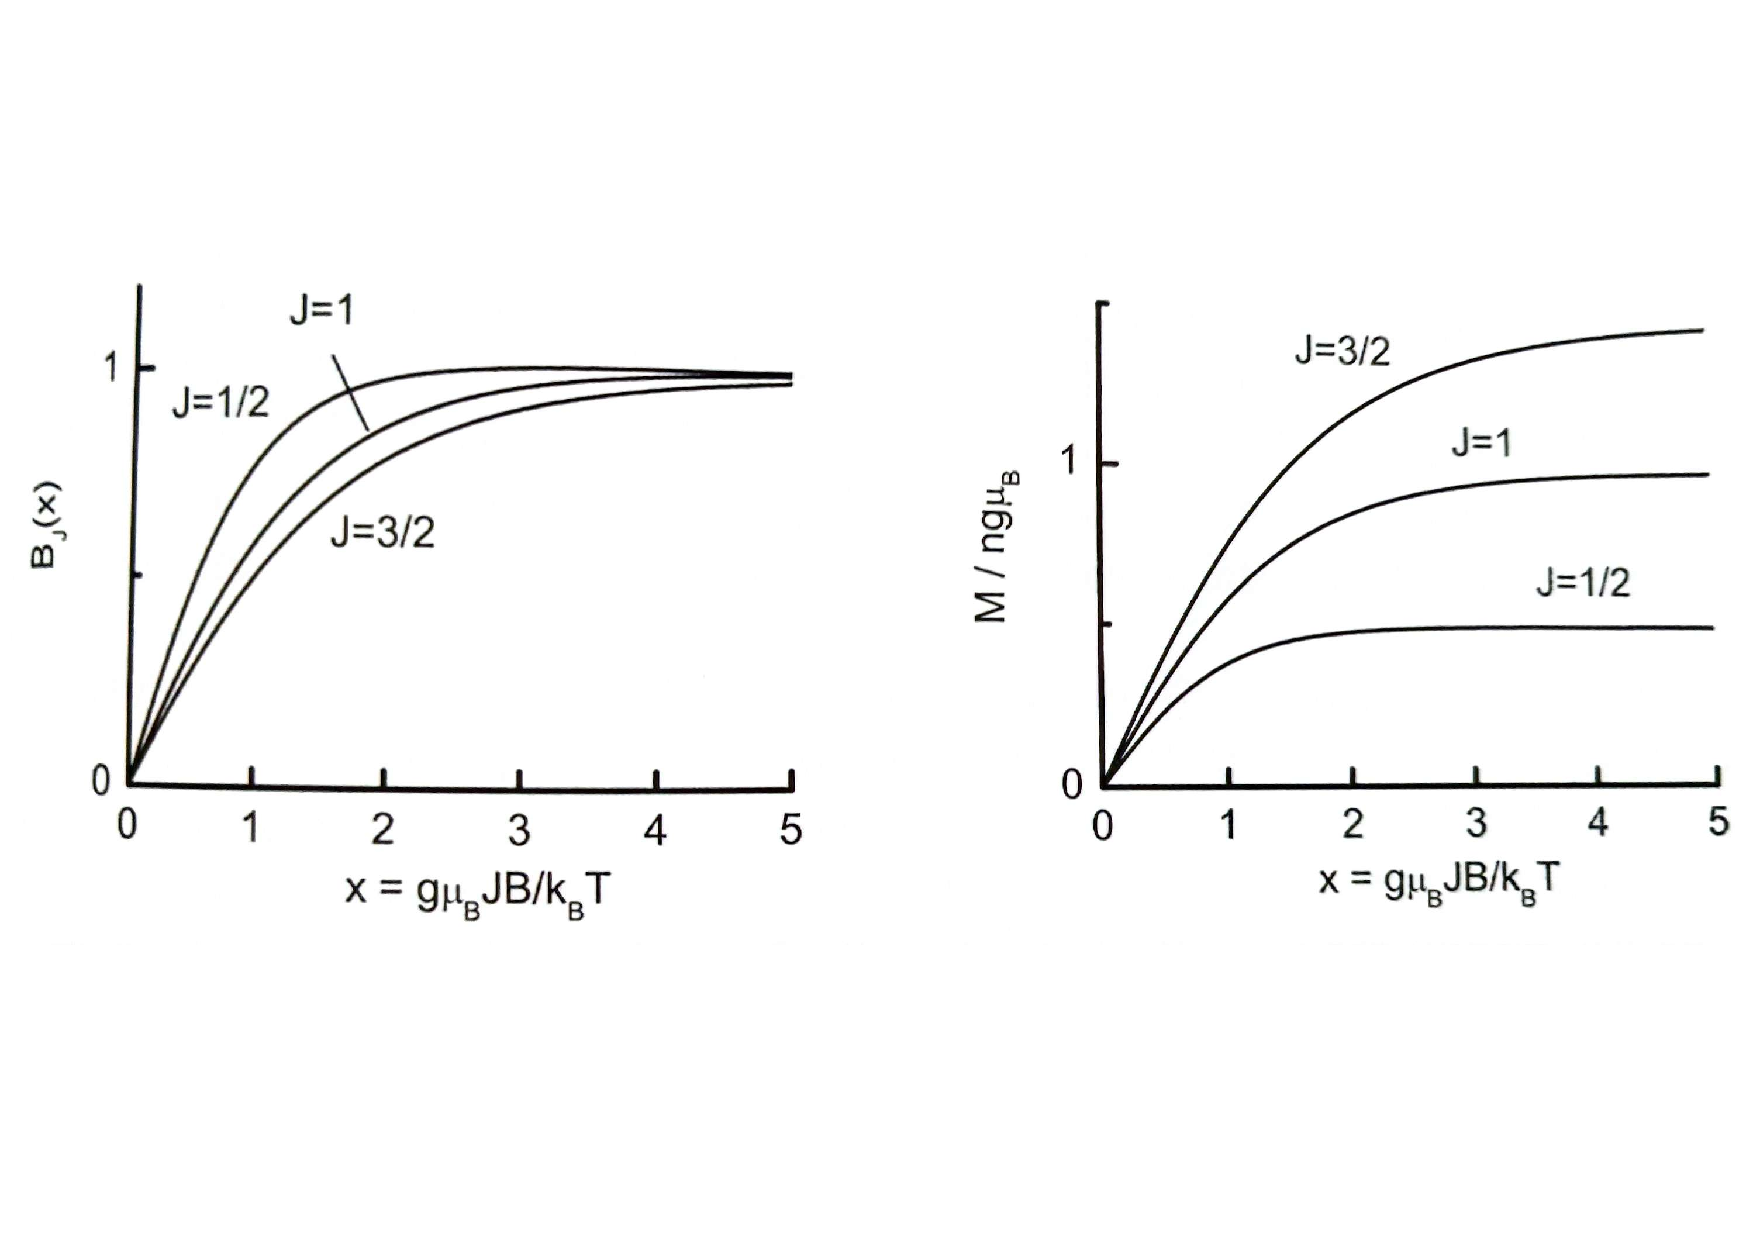
\includegraphics[scale=0.35]{Cuerpo/Ch_10/Fotos libro 2.pdf}
	\caption{Dependencia con $x$ de la función de Brillouin y de la magnetización paramagnética para distintos valores de $J$.}
	\label{Fig:10-02}
\end{figure}

\subsection{Ley de Curie}

A temperatura ambiene, para los campos más altos alcanzables en un laboratorio $(\sim 10$ T) $x\ll 1$, y $B_J(x)$ se aproxima Por

\begin{equation}
	B_J (x) = \frac{J+1}{3J} x
\end{equation}
de modo que la susceptibilidad paramangética es 

\begin{equation}
	\chi = \frac{M}{H} \approx \frac{mu_0 M}{B} = \frac{nJ(J+1)g^2 \mu_0 mu_B^2}{3k_BT} \label{Ec:10-03-11}
\end{equation}
donde $p=g \sqrt{J(J+1)}$ es el \textit{número efectivo de magnetos de Bohr}. La relación (\ref{Ec:10-03-11}) se denomina \textbf{ley de Curie} y a $C$ se le denomina \textit{constante de Curie}. Numéricamente se encuentra que $\chi\sim 10^{-3}$, lo que justifica la aproximación $B=\mu_0 (H+M) \approx \mu_0 H$. Es destacable que, aunque pequeña, es $10^2-10^3$ veces mayor que la correspondiente a la contribución diamangética.

% tabla 

La tabla muestra la comparación entre el valor de $p$ teórico y el experimental determinado por el coeficiente en $1/T$ de la susceptibilidad medida para un conjunto de iones de tierras raras (capa $f$ interna incompleta). El acuerdo es muy  bueno excepto para el Eu para el que como $J=0$, habría que que considerar la contribución a $M$ en (\ref{Ec:10-03-07}) de otros multipletes (estados excitados con distinto $J$). La situación es muy distinta para los iones de los elementos de transición (capa $d$ externa incompleta), como se muestra en la tabla , donde aunque se verifica la ley de Curie sólo hay acuerdo si se admite que $L=0$. Se interpreta esta anulación del momento angular orbital como un efecto producido por los iones vecinos, siendo afectadas las capas electrónicas $d$ por el campo eléctrico que estos generan (a esto lo llamamos \textit{efecto de campo cristalino}). Éste, sin embargo, no afecta a las tierras raras pues la capa interna $f$ está mucho más cerca del núcleo y protegida del campo ``ambiental'' por las capas $5s$ y $5p$.

% tabla

\section{Paramagnetismo de los electrones de conducción}

Los resultados anteriores no son válidos para los electrones de conducción pues por el principio de exclusión no se pueden considerar independientes, que es lo que hemos admitido en la sección anterior. En efecto, vamos a ver cómo el principio de Pauli limita fuertemente el alineamiento de los espines electrónicos con el campo. La figura \ref{Fig:10-03} muestra cómo actúa un campo magnético $B$ sobre el mar de Fermi.

\begin{figure}[h!] \centering
	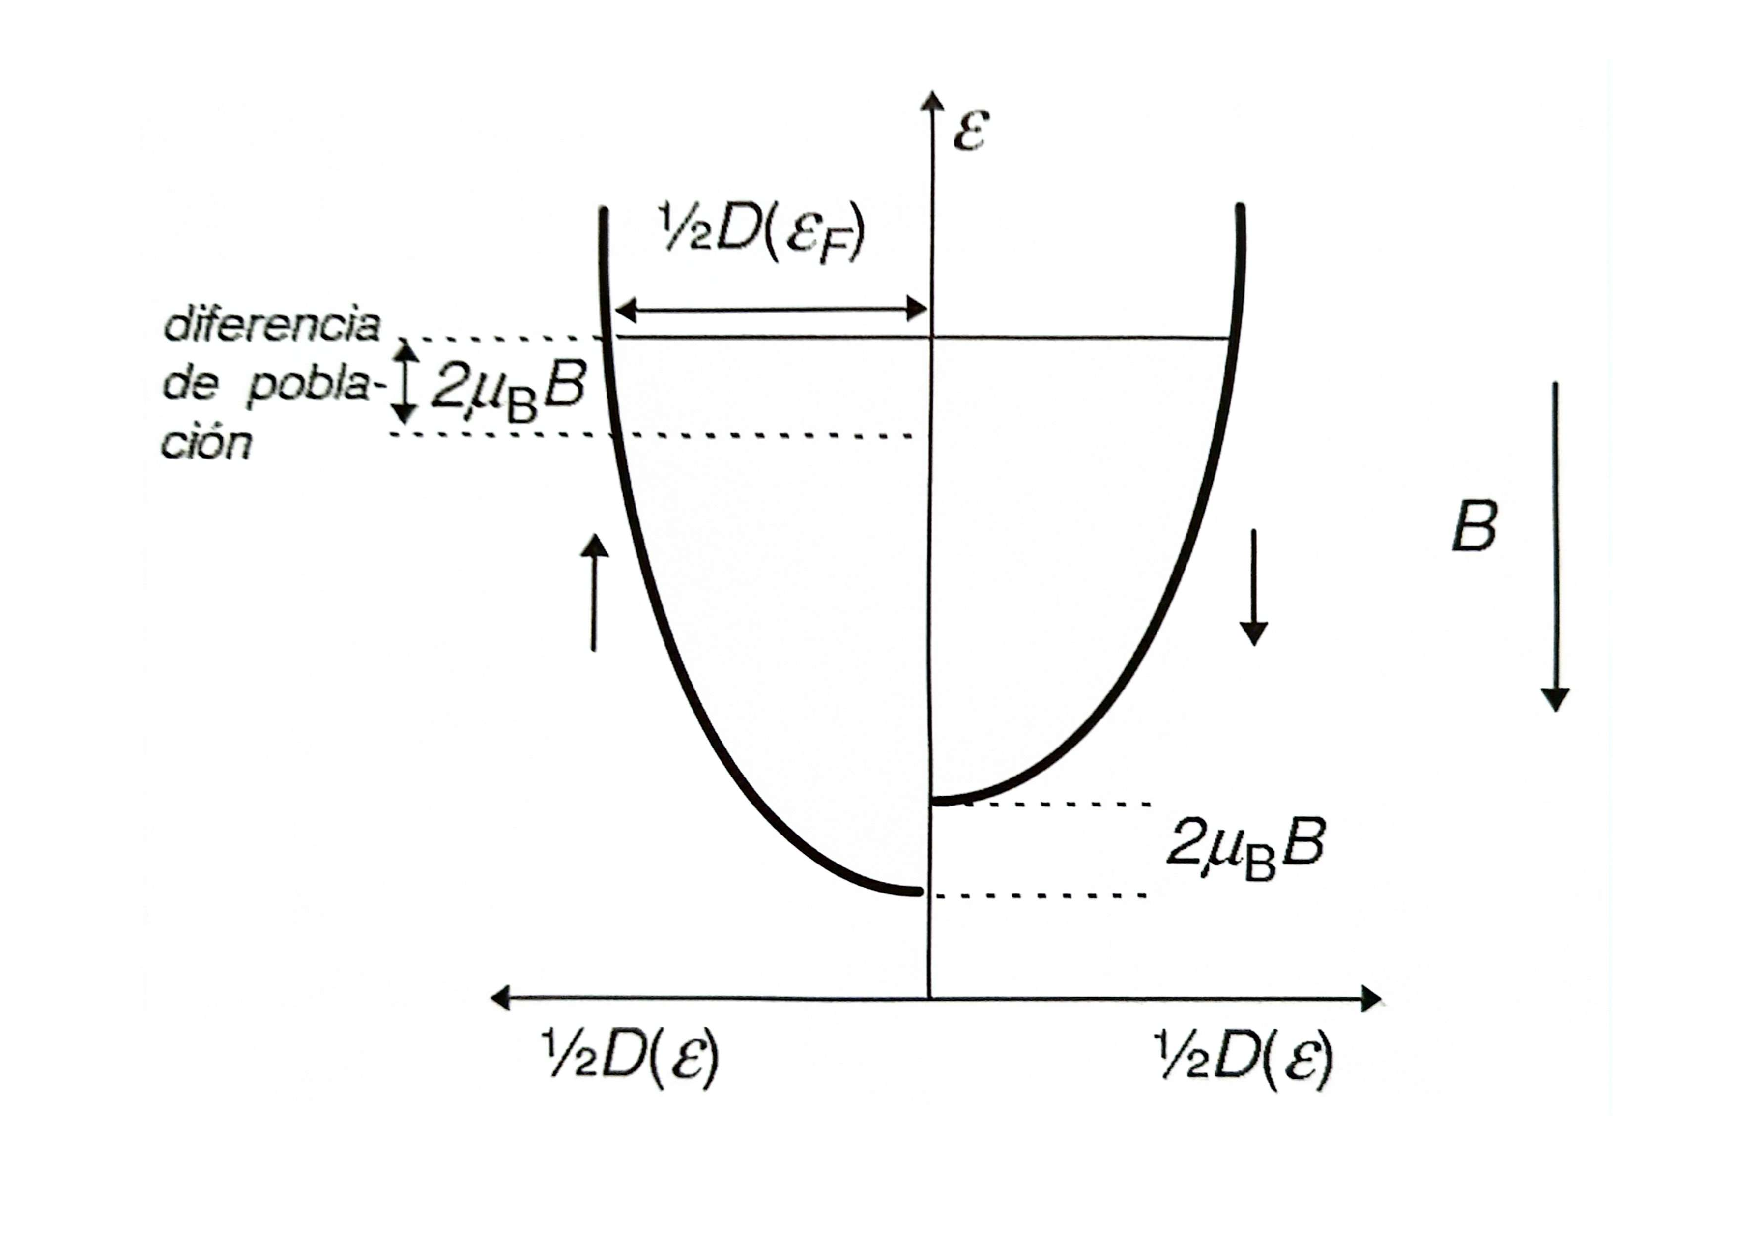
\includegraphics[scale=0.35]{Cuerpo/Ch_10/Fotos libro 3.pdf}
	\caption{Desplazamiento relativo de los niveles energéticos electrónicos correspondientes a espín $\uparrow$ y espín $\downarrow$.}
	\label{Fig:10-03}
\end{figure}

Como $S=\pm 1/2$, por (\ref{Ec:10-03-02}) se tiene $\mu=\mu_B$, de modo que las energías electrónicas se corren en $\pm \mu_B B$ según la orientación del momento magnético de espín. La diferencia en la concentración de electrones con espín $\uparrow$ y $\downarrow$, $\Delta n$, es igual al área de la proporción rectangular indicada (observar también que la condición de equilibrio exige que el potencial químico $\varepsilon_F$ sea el mismo para ambos grupos de espines). Como para los mayores campos alcanzables $\mu_B B \ll \varepsilon_F$ (por ejemplo, $\mu_B B \approx 0.6 $ meV a $B=10$ T), el área se aproxima por $\Delta n \approx \frac{1}{2} D (\varepsilon_F) 2 \mu_B B$. Utilizando que para electrones libres $D(\varepsilon_F) = 3n/2\varepsilon_F = 3n/2k_B T_F$ resulta 

\begin{equation}
	M= \mu_B \Delta n = \frac{3n\mu_B^2}{2k_B T_F} B
\end{equation}


\section{La interacción de intercambio}

\section{Ferromagnetismo}

\section{Dominios ferromagnéticos}

\section{Orden ferrimangnético}

\begin{figure}[h!] \centering
	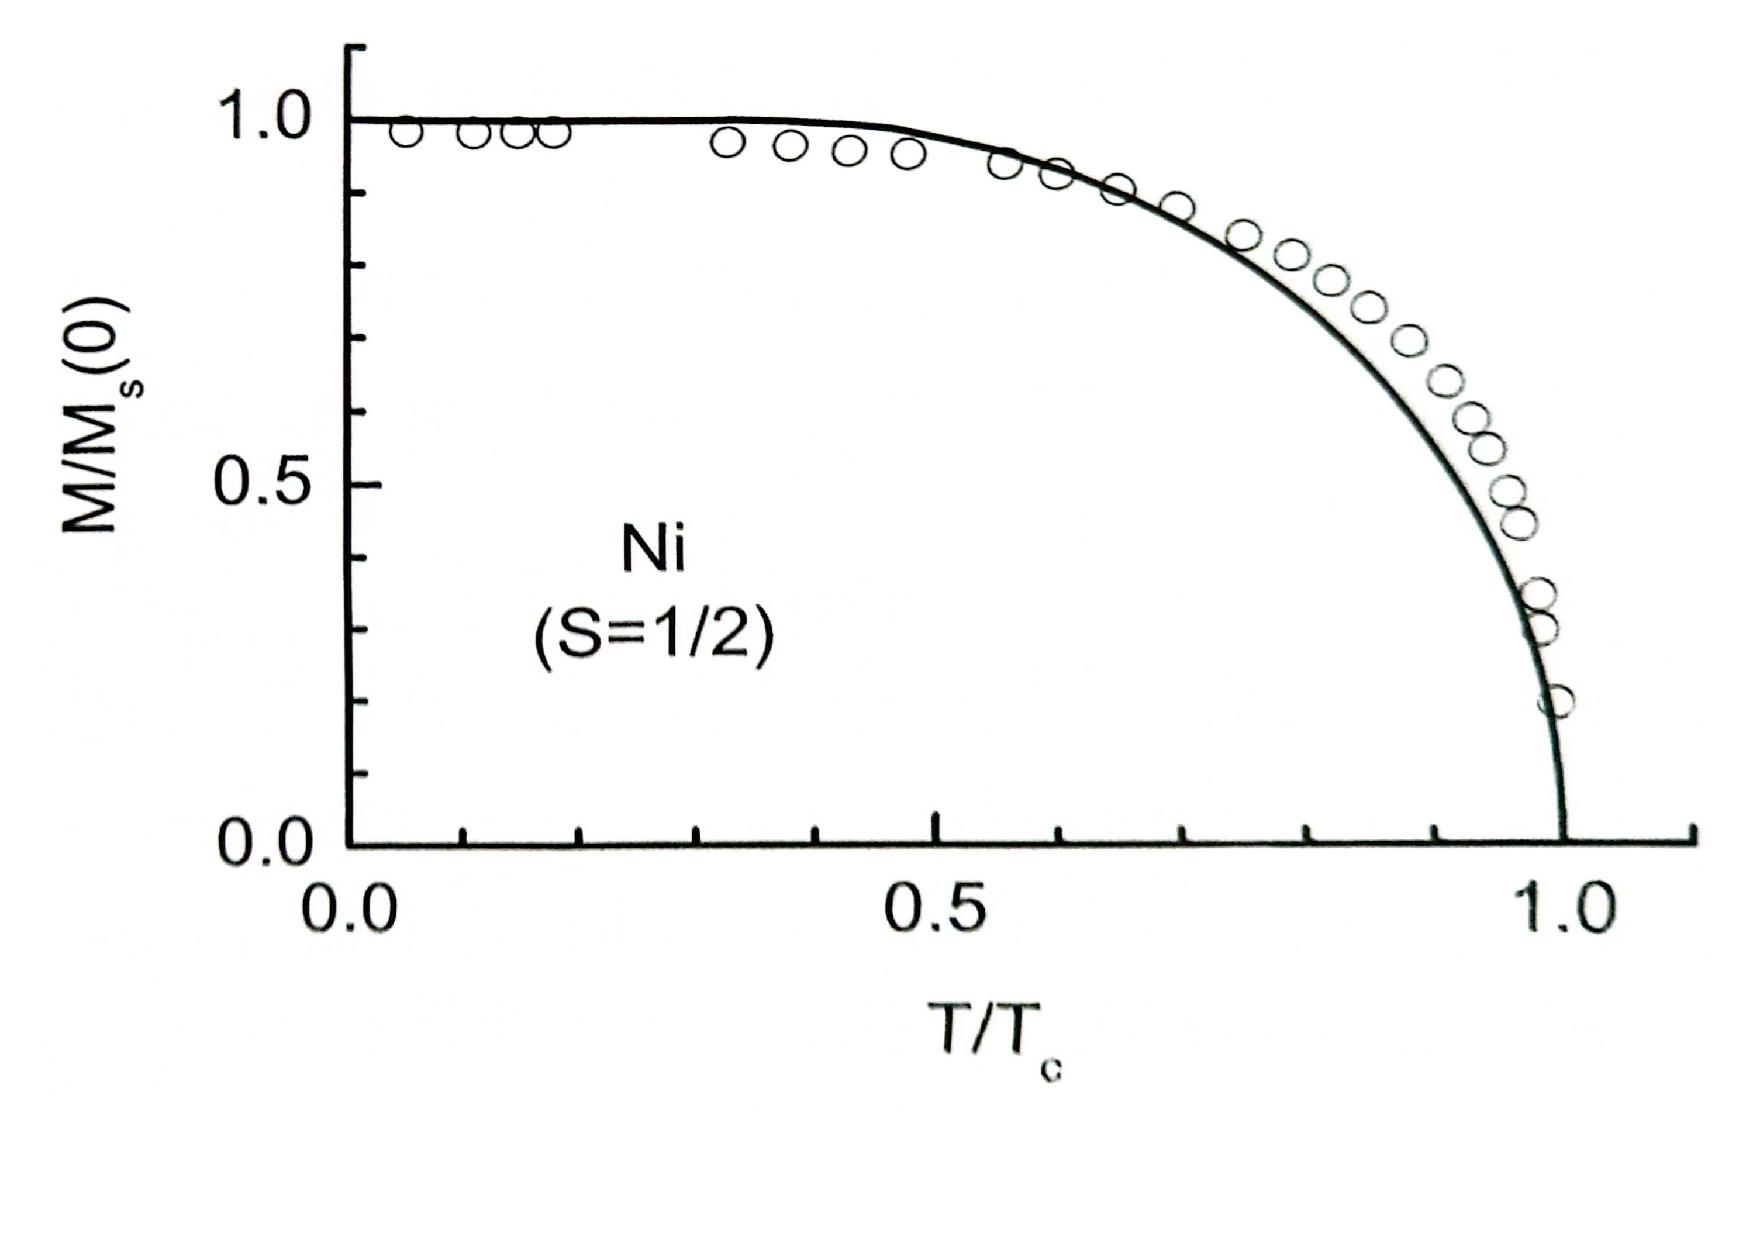
\includegraphics[scale=0.35]{Cuerpo/Ch_10/Fotos libro 4.pdf}
	\caption{Dependencia con la temperatura de la magnetización espontánea para el Ni cuando $T<T_C$, y compensación con las predicciones de campo medio.}
	\label{Fig:10-04}
\end{figure}
\begin{figure}[h!] \centering
	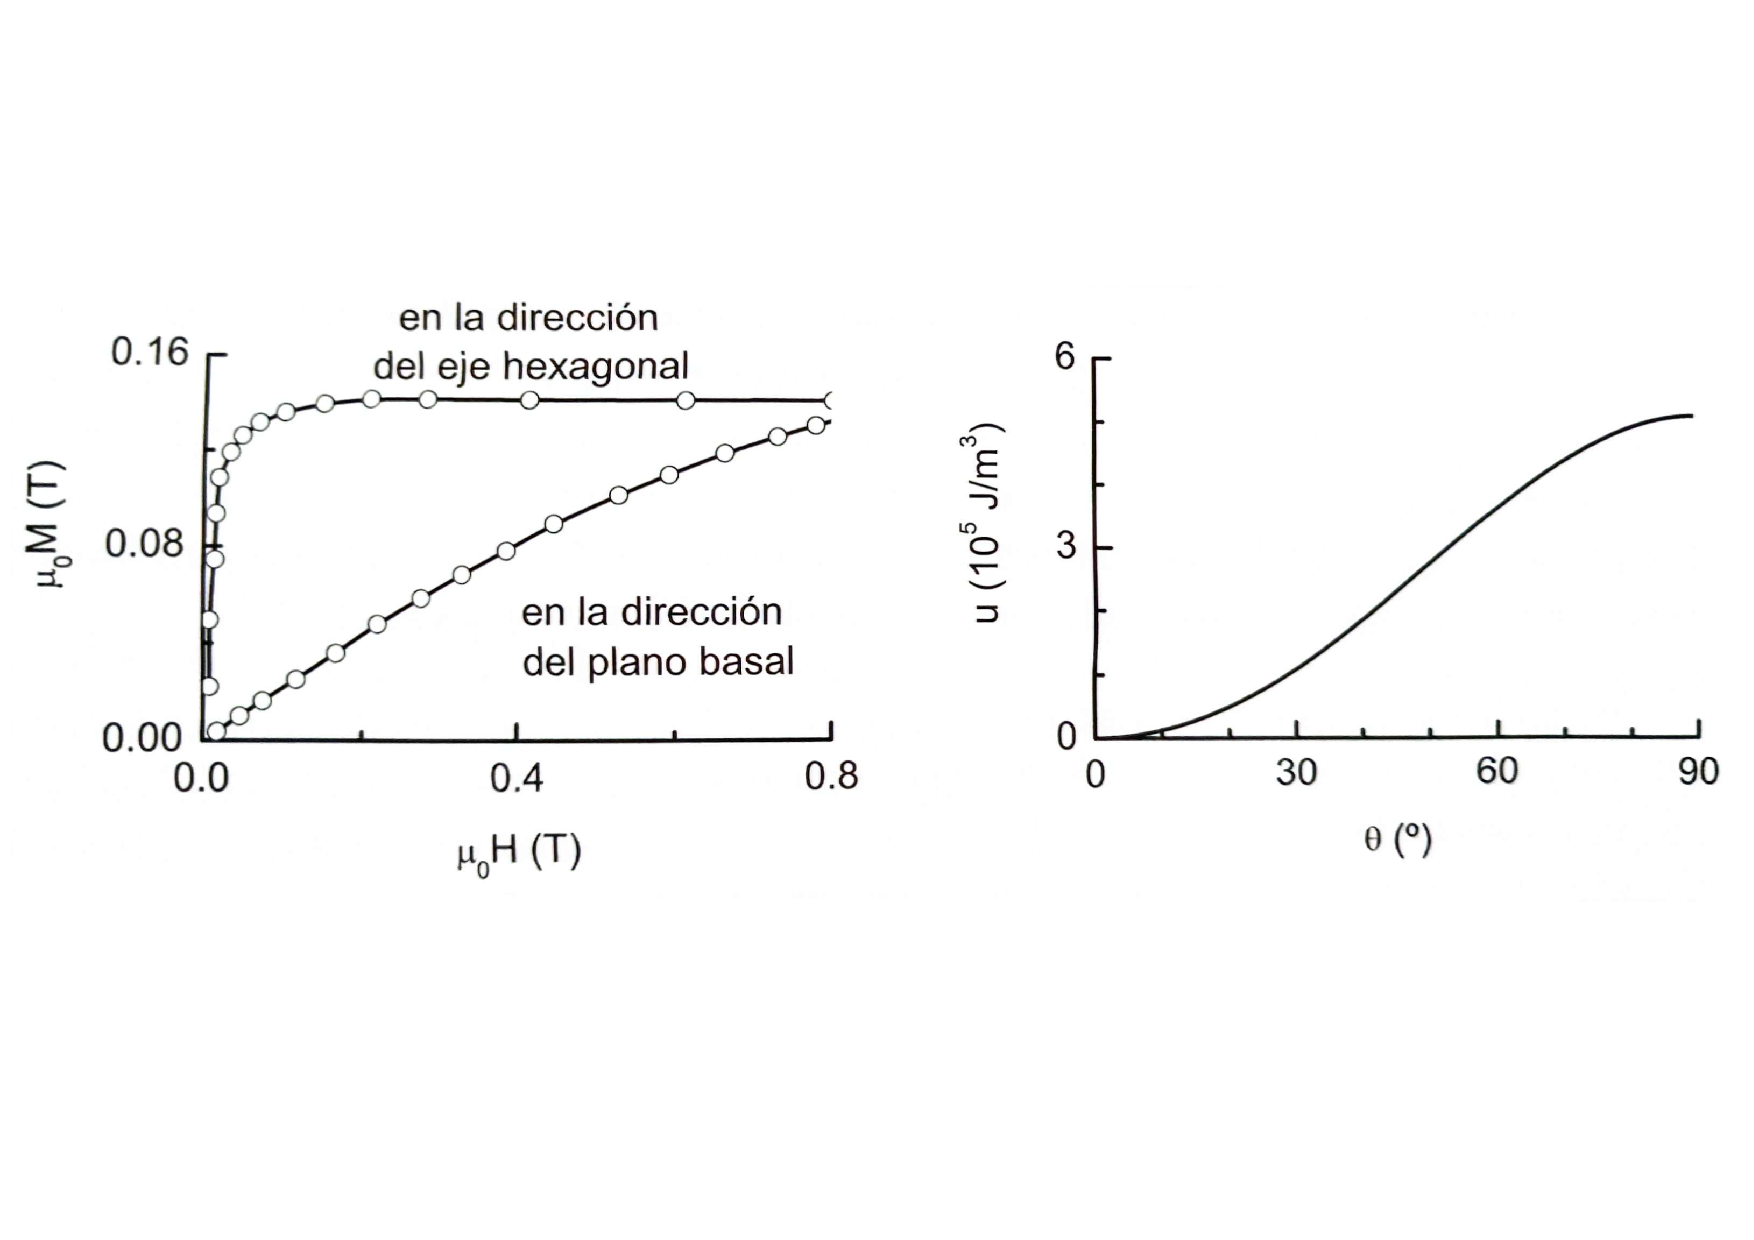
\includegraphics[scale=0.35]{Cuerpo/Ch_10/Fotos libro 5.pdf}
	\caption{En la izquierda la magnetización de una muestra de  Co para las direcciones paralela y perpendicular al plano basal de la estructura hexagonal. En la derecha de anisotropía del Co según el ángulo que forma la magnetización con el eje hexagonal.}
	\label{Fig:10-05}
\end{figure}
\begin{figure}[h!] \centering
	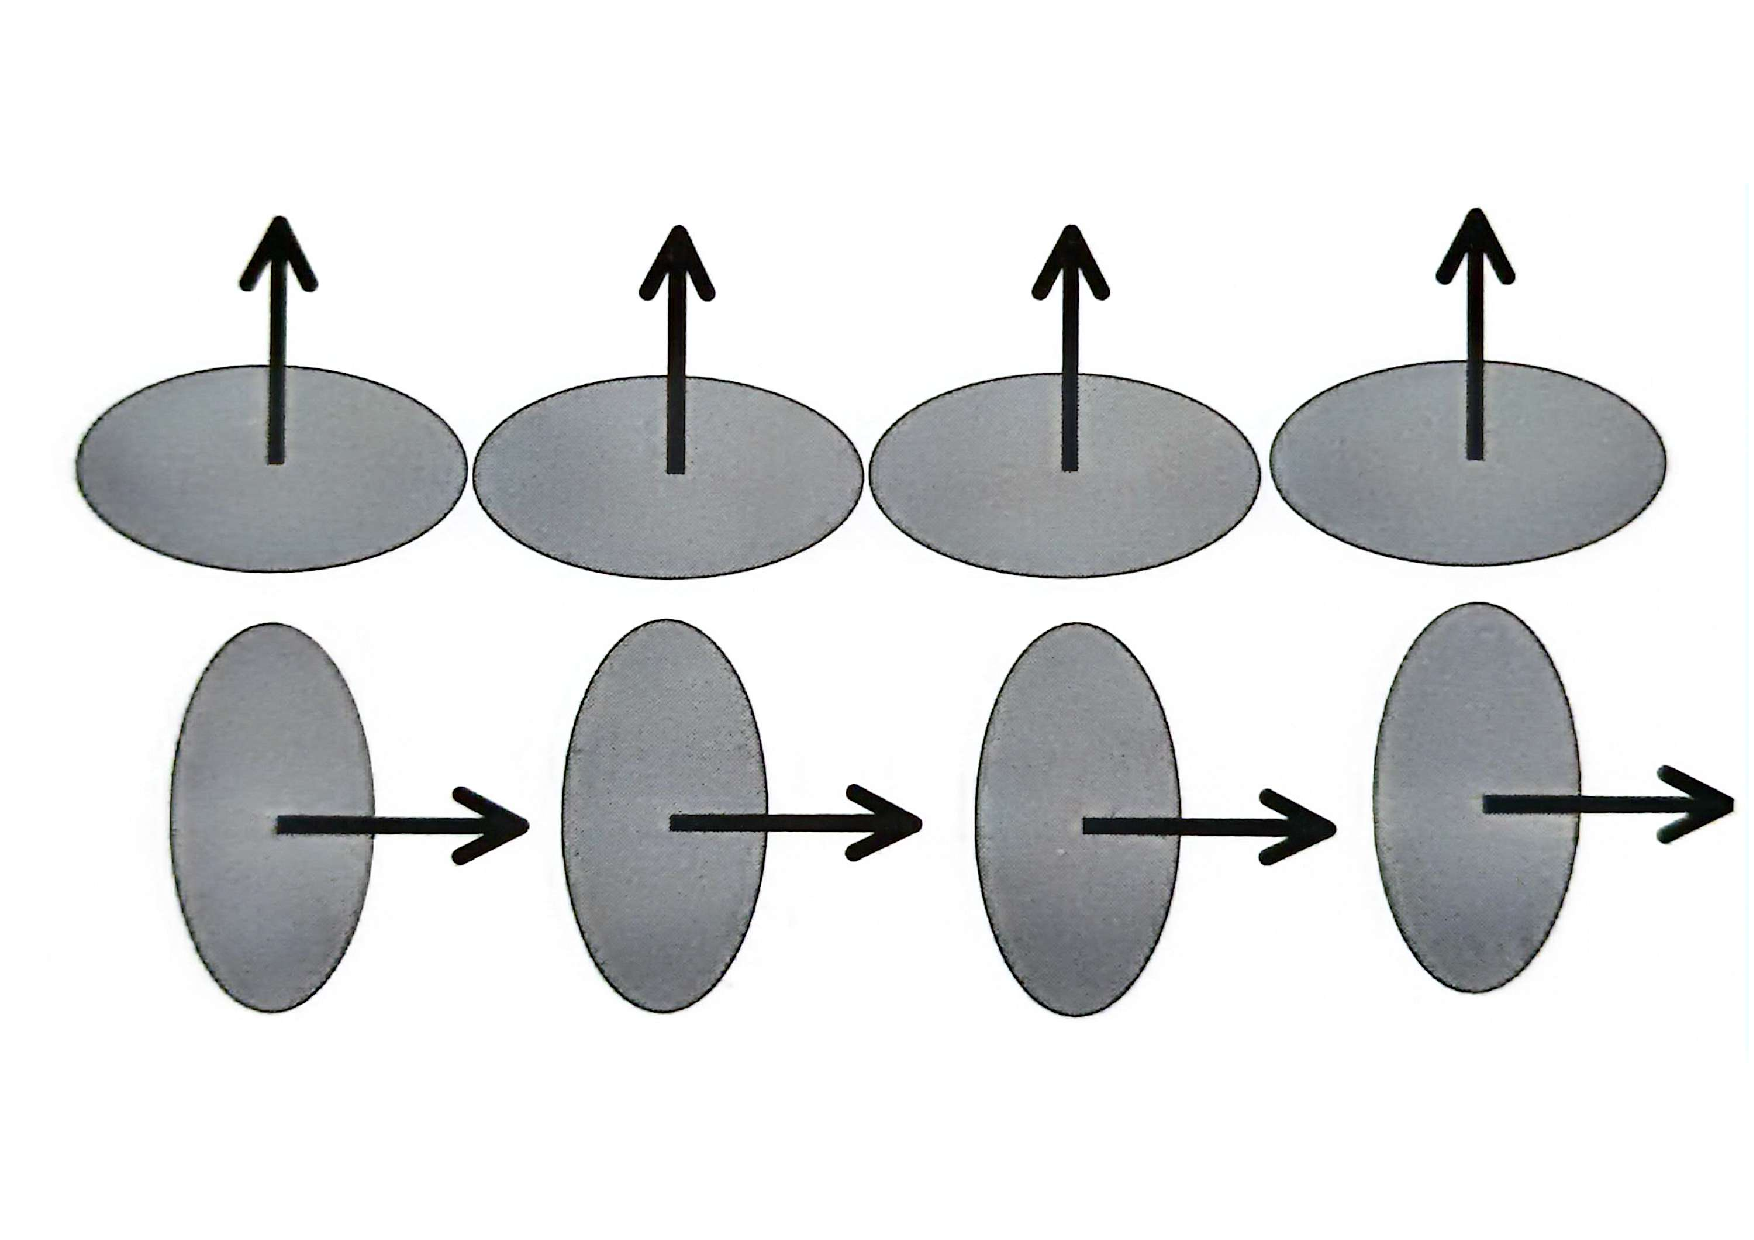
\includegraphics[scale=0.35]{Cuerpo/Ch_10/Fotos libro 6.pdf}
	\caption{Distribución electrónica para diferntes orientaciones del campo mangético aplicado.}
	\label{Fig:10-06}
\end{figure}
\begin{figure}[h!] \centering
	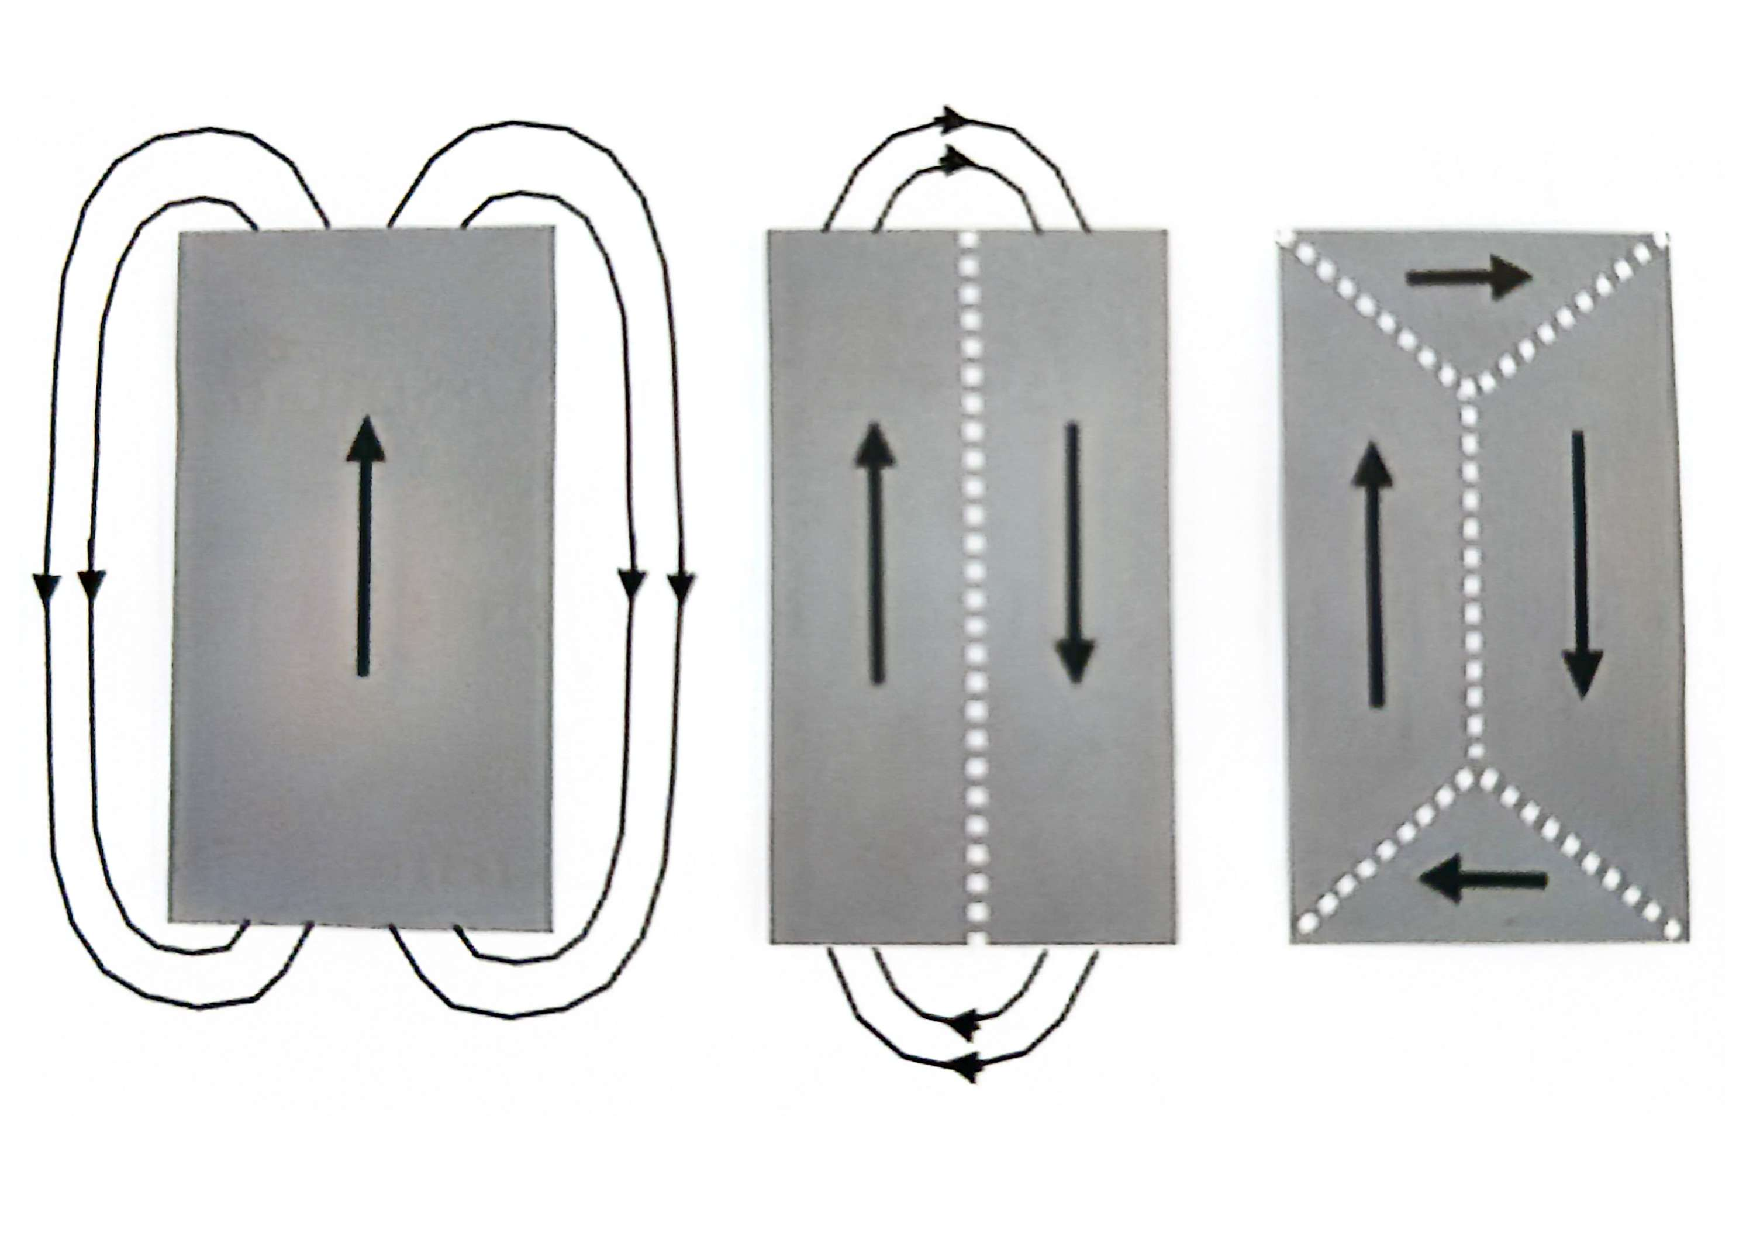
\includegraphics[scale=0.35]{Cuerpo/Ch_10/Fotos libro 7.pdf}
	\caption{Aparición de dominios en una muestra ferromagnética. Las flechas indican la orientación de los momentos magnéticos en cada dominio.}
	\label{Fig:10-07}
\end{figure}
\begin{figure}[h!] \centering
	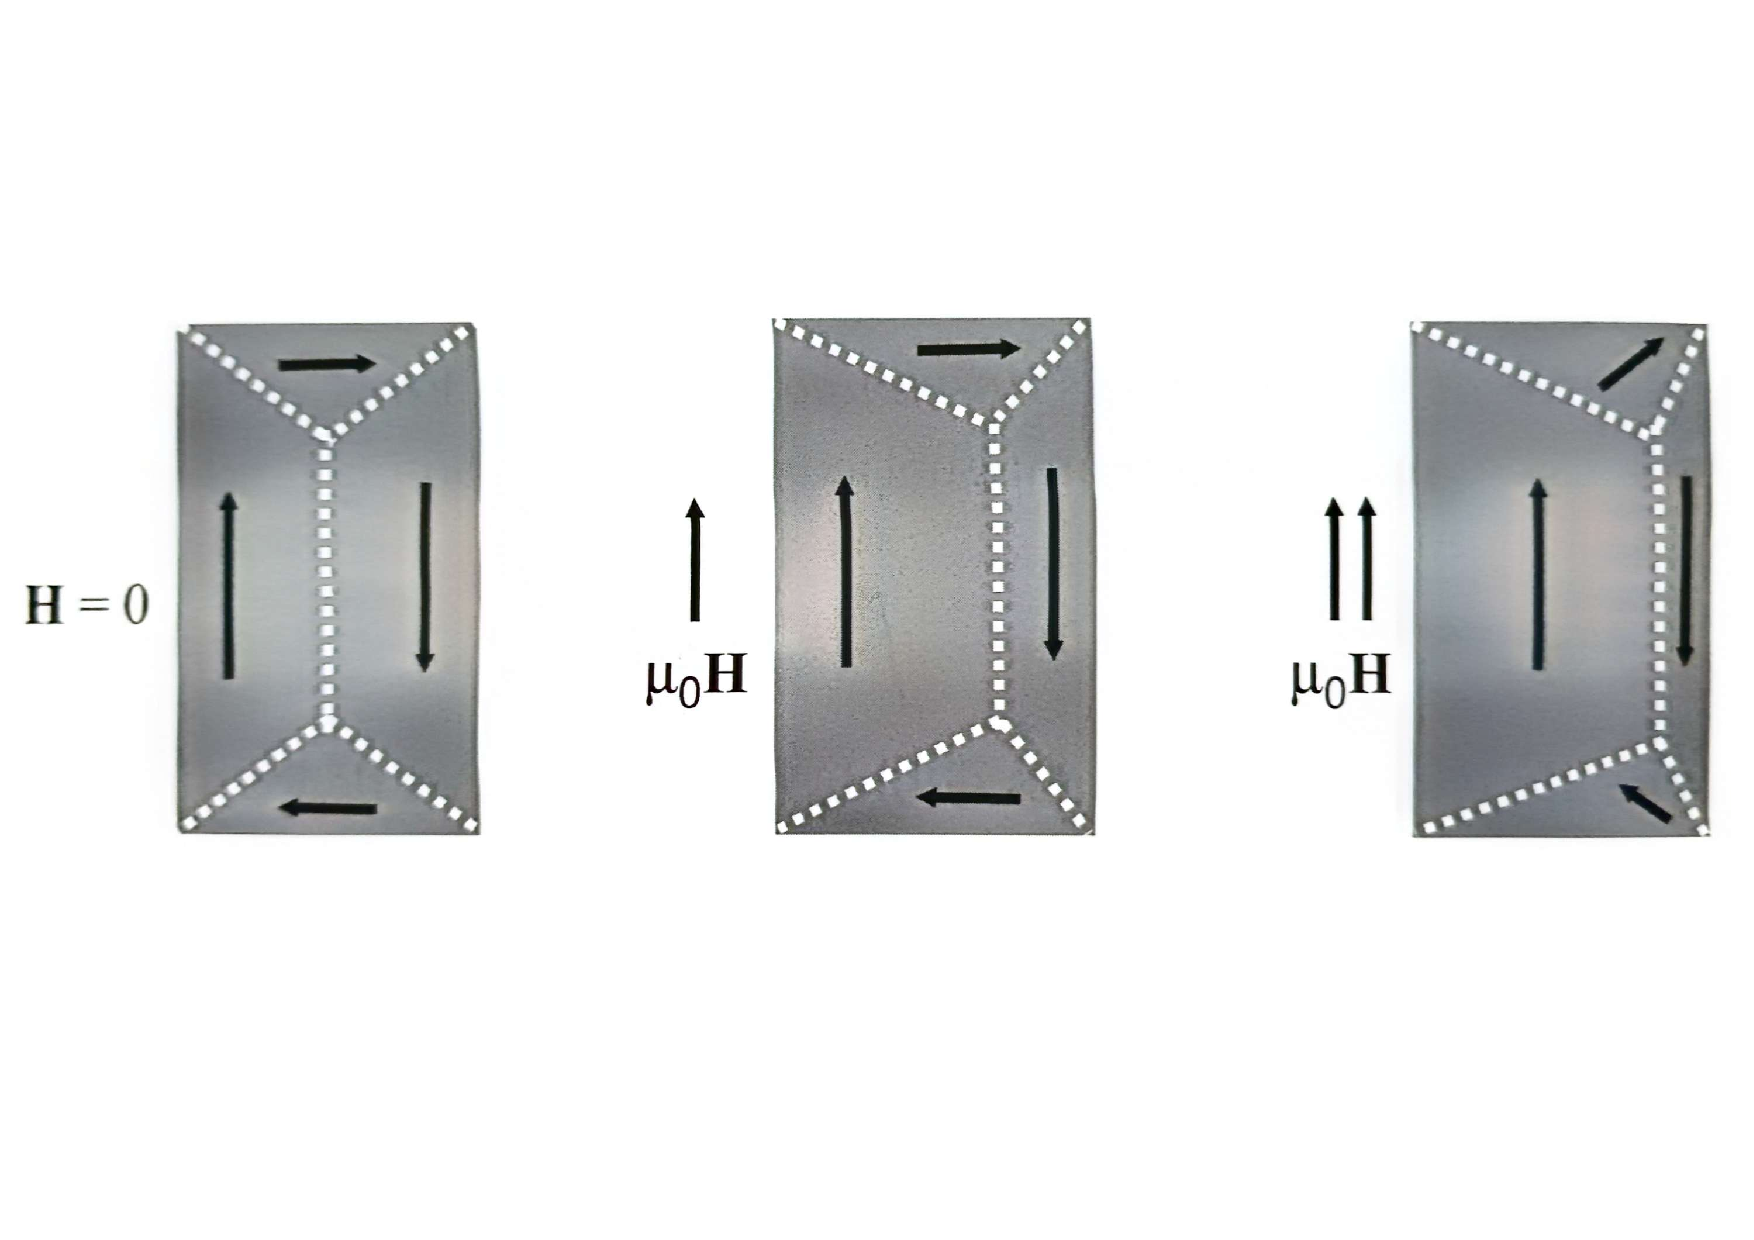
\includegraphics[scale=0.35]{Cuerpo/Ch_10/Fotos libro 8.pdf}
	\caption{Desplazamiento de las fronteras entre dominios debido a una variación del campo magnético aplicado.}
	\label{Fig:10-08}
\end{figure}
\begin{figure}[h!] \centering
	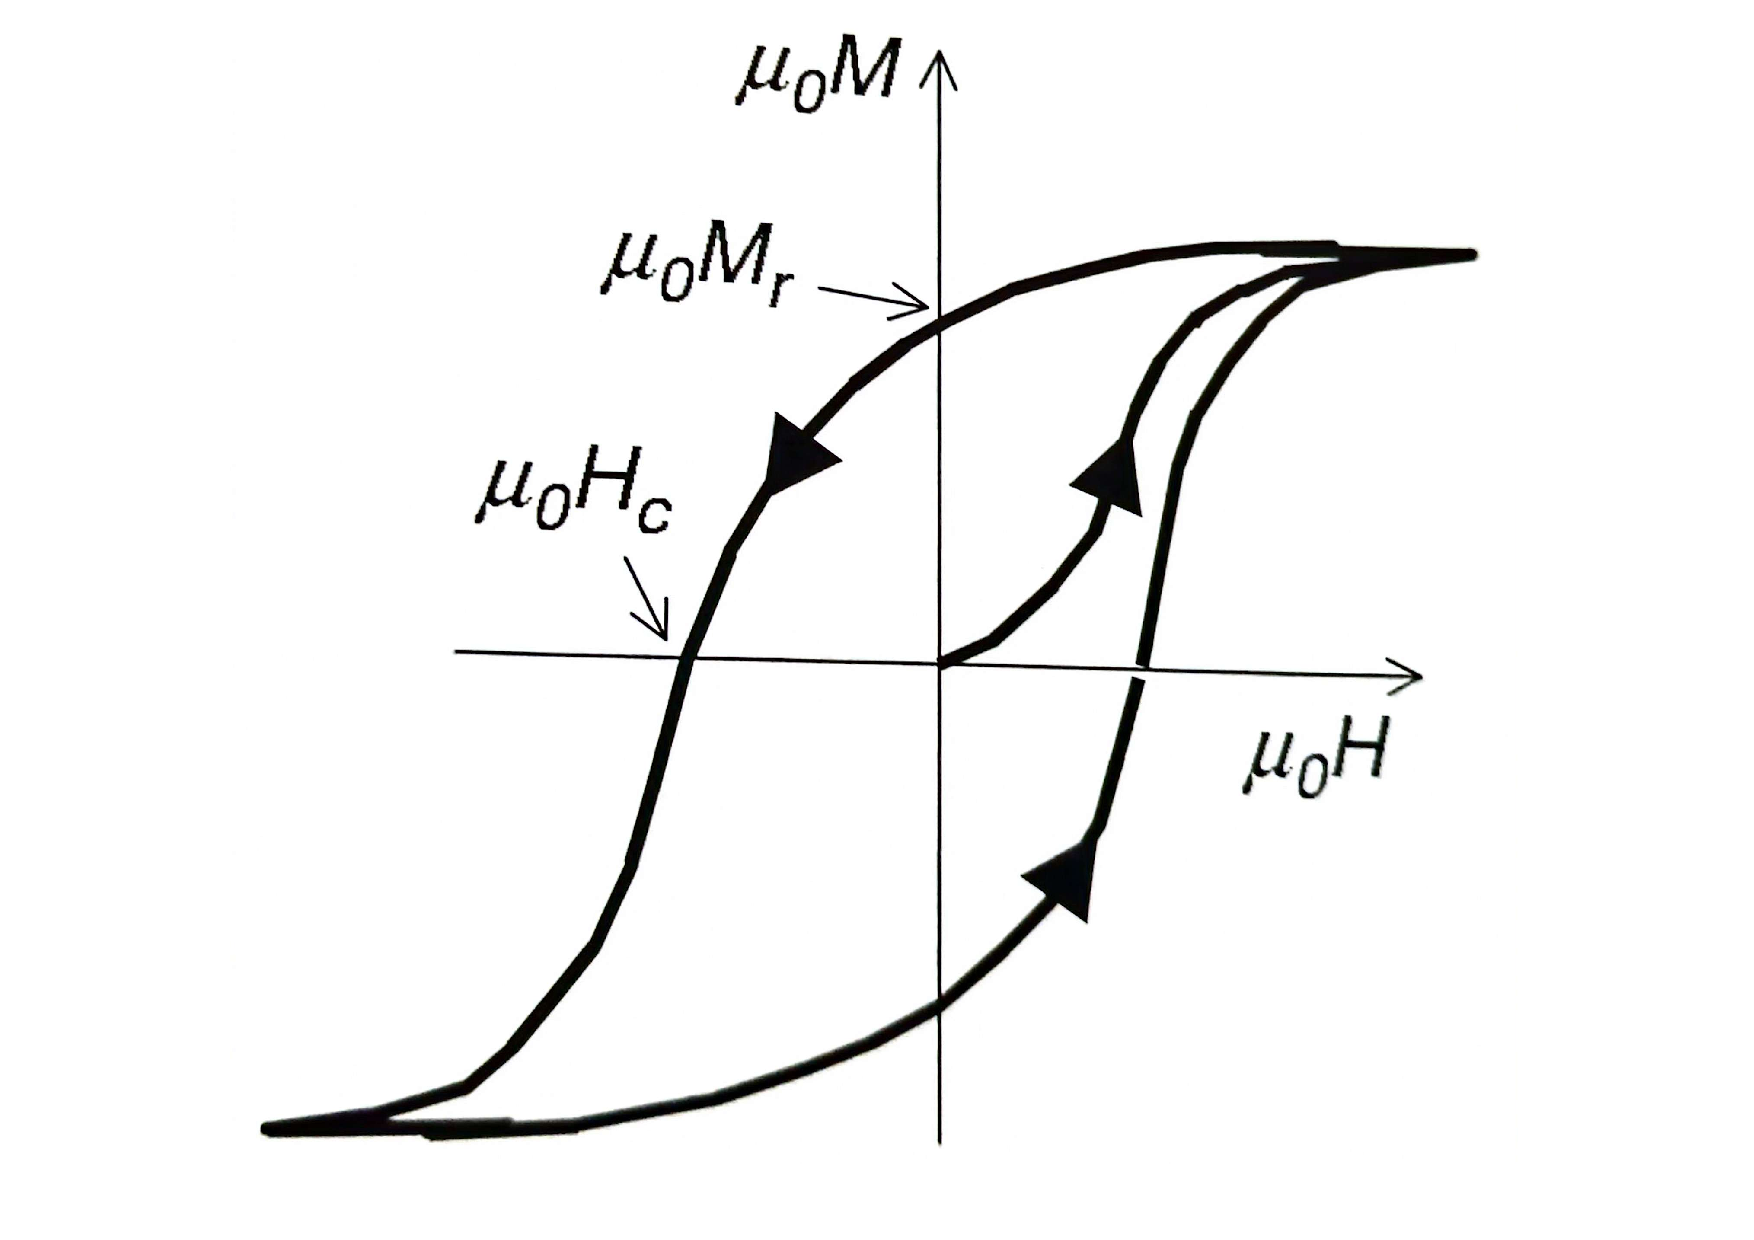
\includegraphics[scale=0.35]{Cuerpo/Ch_10/Fotos libro 9.pdf}
	\caption{Histéresis de la dependencia $M(H)$ debida al anclado de las paredes Bloch en los defectos del material.}
	\label{Fig:10-09}
\end{figure}